\section{Scaffolding Engagements through \ONT{}'s Design Vocabulary}
\label{section:scenarios}

This section will use the visual design vocabulary to describe and demonstrate the use of \ONT{} with three different archetypes of group interactions: talk shows, research workshops, and speed dating events. 

\subsection{Scenario 1: Talk Show}

\begin{figure}[h]
  \centering
  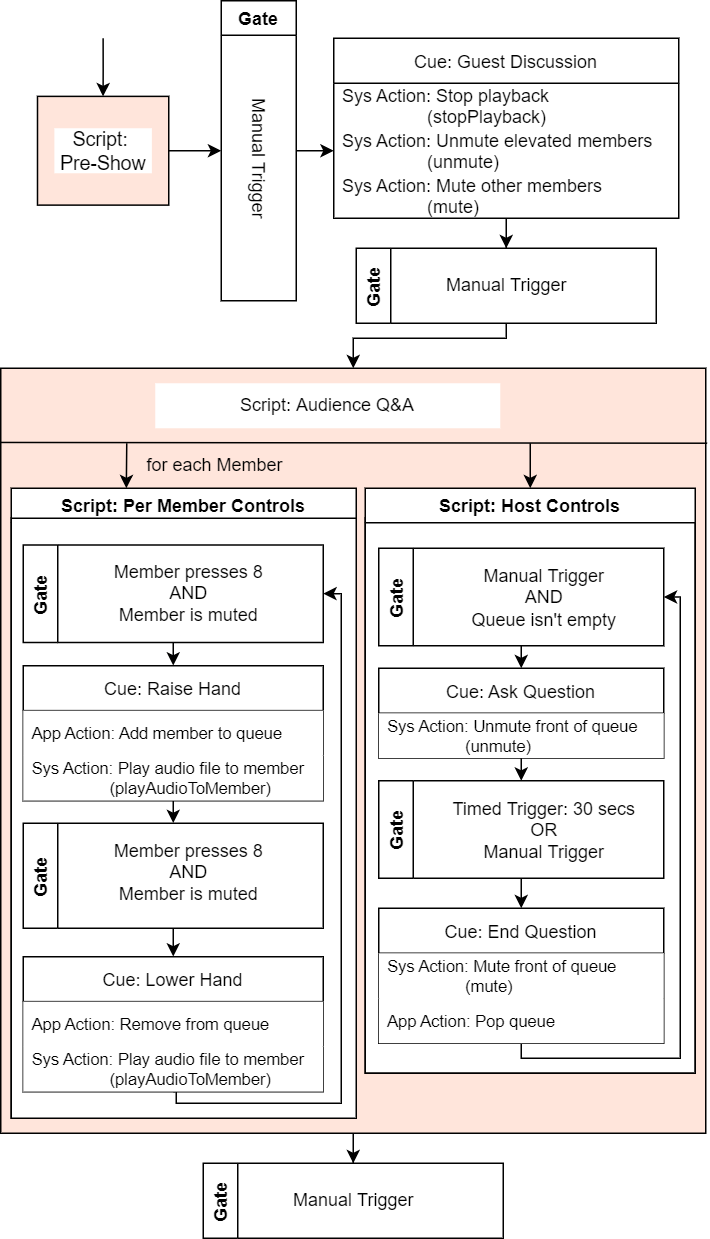
\includegraphics[width=0.5\columnwidth]{images/example_talkshow.drawio.png}
  \Description{Another flow chart style diagram, showing how a talk show could be implemented in \ONT{}. The first item is a Script labelled 'pre-show', referencing the previous diagram. This is followed by a Gate containing a Manual Trigger Condition. This is then followed by a Cue titled 'Guest Discussion', which has three System Actions: stop playback of playing audio files, unmute the elevated user group, and mute other members. This Cue is followed by another Gate with a Manual Trigger, which leads to another Script, titled 'Audience Q\&A'. This Script can be interrupted by a Manual Trigger, and contains two looping tracks of logic. The first, labelled 'for each member', features a Script titled 'per member controls'. The first item in this script is a Gate, with the conditions 'member presses 8' and 'member is muted', connected with the 'AND' operator. This gate is followed by a Cue titled 'raise hand', which has the App Action 'add member to queue' and a System Action 'play audio to member'. This is then followed by a Gate with the same conditions as before, which leads to a second cue titled 'lower hand'. This Cue has an App Action 'remove from queue' and another play audio to member System Action. It connects to the first Gate, forming a loop. The second track of logic in the parent 'Audience Q\&A' Script has a Script titled 'Host Controls'. This starts with a Gate containing a Manual Trigger and a 'queue isn't empty' contextual trigger, connected by the AND operator. This is followed by a Cue titled 'ask question', which has an unmute System Action labelled 'unmute front of queue'. This is then followed by another Gate, which has two conditions connected by the OR operator: a 30 seconds Timed Trigger, and a Manual Trigger. This Gate is followed by another Cue, titled 'end question', which contains a mute System Action ('mute front of queue') and an App Action ('pop queue'). This Cue is then connected to the first gate in the 'Host Controls' Script, forming a loop.}
  \caption{Using \ONT{} to prototype the interactions involved in a talk show with an audience Q\&A segment. The `Pre-Show' Script is detailed in Figure \ref{fig:preshow}. During the Q\&A, multiple Scripts are active at once: one for the Host, and one for each Member. Note that the handling of race conditions has been omitted to save space.}~\label{fig:talkshow}
\end{figure}

Figure \ref{fig:talkshow} shows how a talk show engagement format (described in Section \ref{section:talkshow}) with strict time-keeping can be scaffolded programmatically using \ONT{}. The main segments of the show (pre-show, guest discussion, and audience Q\&A) are transitioned between by the host through the use of Manual Triggers. The use of containerisation means that the `pre-show' Script previously shown in Figure \ref{fig:preshow} can be re-used. The `guest discussion' unmutes the Elevated Members group (i.e. the host and guests), and mutes everyone else. The `audience Q\&A' Script has two sets of asynchronous tracks: one which is used on a per-Member basis, letting callers add and remove themselves from the queue to ask questions through a button press; and one for the host to manage the queue. When triggered by the host, the Member at the front of the queue will be unmuted for 30 seconds (or manually interrupted by the host) to ask a question, before being muted again and removed from the queue. The Script is exited by a Manual Trigger, after which further logic could either end the show, or clear the queue and ensure that all participants are muted again before continuing. Planning the interaction through \ONT{} and observing used LogicItems shows that this system would need to implement mute, unmute, and audio playback SystemActions, as well as a queue system which can be manipulated by callers and the host.


\subsection{Scenario 2: Research Workshop}

\subsubsection{Overview}

Since the start of the COVID-19 pandemic, it has become more common to hold research workshops remotely though platforms such as Zoom: the `breakout room' feature (where callers can be temporarily subdivided into smaller discussion groups) can be used as an analogue for having separate tables of participants within a qualitative workshop to support group discussion and activities. This degree of dynamic manipulation of call topology has not yet been supported within existing synchronous group telephony platforms.

\begin{figure}[h]
  \centering
  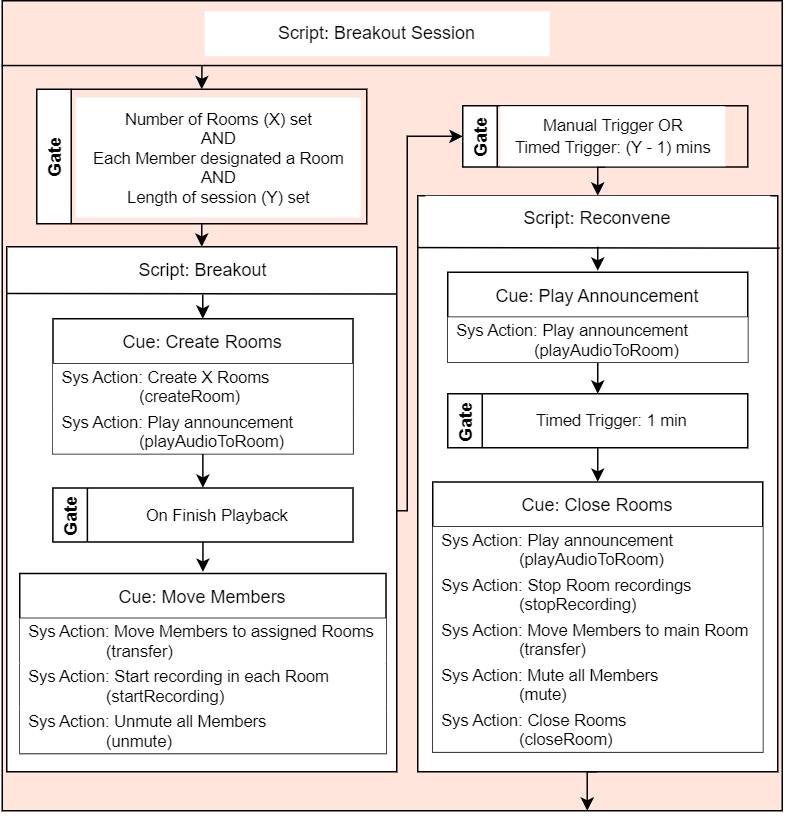
\includegraphics[width=0.5\columnwidth]{images/example_workshop.drawio.png}
  \Description{}
  \caption{Using \ONT{} to scaffold a `breakout room' interaction to be used during a distributed research workshop}~\label{fig:breakout}
  \Description{Another flow chart style diagram, showing how a breakout room interaction could be implemented in \ONT{} to facilitate a research workshop scenario. It consists of a 'Breakout Session' Script containing two gates and two nested scripts. It starts with a Gate with three conditions: 'number of rooms (X) set', 'each member designated a room', and 'length of session (Y)'; all connected with the 'AND' operator. Within these conditions, X and Y are previously set variables. This Gate is followed by a nested Script labelled 'Breakout', which starts with a Cue titled 'Create Rooms'. This cue has two System Actions: create X number of rooms and play announcement audio to the (main) room. This is followed by a Gate with the condition 'On Finish Playback', which connects to another Cue titled 'Move Members'. This Cue has three System Actions: move members to assigned rooms, start recording in each room, and unmute all members in the rooms. The 'Breakout' Script terminates with a Gate containing two conditions connected by the 'OR' operator: a Manual Trigger condition and a Y-1 minutes Timed Trigger (the length of session, Y, minus one minute). The Gate links to the next nested Script labelled 'Reconvene', which starts with a Cue titled 'Play Announcement'. This has one play audio to room System Action. This is followed by a Gate that contains a one minute Timed Trigger, followed by the final Cue within the 'Reconvene' Script titled 'Close Rooms'. The 'Close Rooms' Cue has five System Actions: play announcement audio to the rooms, stop room recordings, move members back to main room, mute all members, and close all (breakout) rooms. After completing the reconvene script, the parent breakout session script exits.}
\end{figure}

\subsubsection{\ONT{} Implementation}

Figure \ref{fig:breakout} shows how \ONT{} could be used to scaffold a `breakout' segment of a research workshop though synchronous telephony (answering \textit{CQ3}). Prior to commencing, this Script requires a configuration noting the number of Rooms to create, the length of time the breakout session should run for, and an assignment of which Members should go to each room. The Script will create the given number of Rooms, play a pre-recorded announcement to Members, and then move them to their assigned Room. The system records each room to a separate audio file for later reference by the researchers, who may not be present in all Rooms. When there is one minute left (or the Host intervenes) another announcement is played, and the Members are muted and moved back to the main Room when the timer expires. This interaction requires the PBXService to be able to create Rooms and assign Members to them: within FreeSWITCH (used by \cite{Kazakos2016, Talhouk2017, Yadav2017}), this can be achieved through the use of conferences\footnote{\url{https://freeswitch.org/confluence/display/FREESWITCH/mod\_conference}} and transfers\footnote{\url{https://freeswitch.org/confluence/display/FREESWITCH/mod\_dptools\%3A+transfer}}.


\subsection{Scenario 3: Speed dating}

\subsubsection{Overview}

Speed dating events typically involve a group of individuals being split into pairs to have short, one-on-one conversations, with pairs cycling every few minutes so that all suitably matched participants have a chance to meet. While fairly simple to organise in person, doing such structured interactions remotely through standard telephony would be highly labour intensive and prone to error: likely requiring participants manage their own timings and hold separate phone calls for each pairing.

\begin{figure}[h]
  \centering
  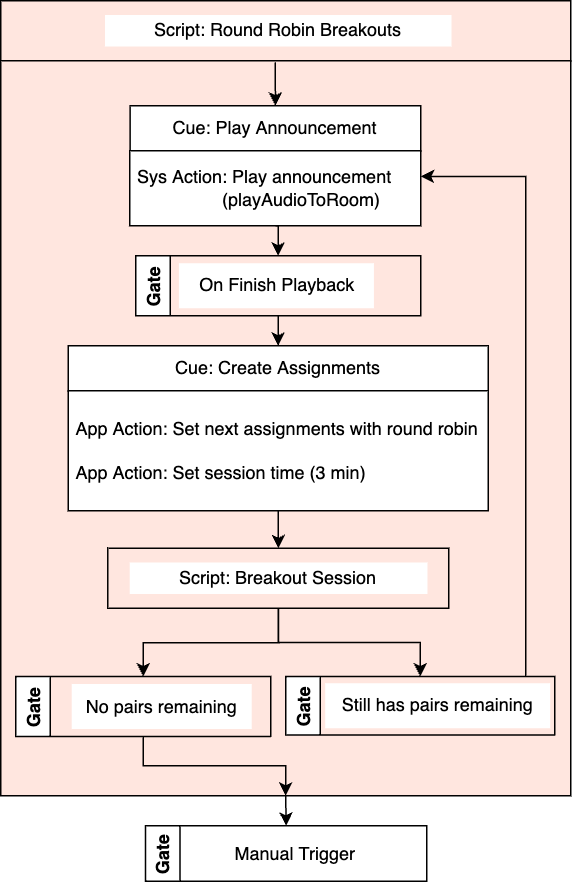
\includegraphics[width=0.4\columnwidth]{images/example_speeddating.drawio.png}
  \Description{}
  \caption{Using \ONT{} to scaffold a `speed dating' interaction using breakout rooms in a round robin configuration. The `Breakout Session' Script can be re-used from Figure \ref{fig:breakout} with minimal modification.}~\label{fig:roundrobin}
  \Description{Another flow chart, detailing a Script labelled 'Round Robin Breakouts'. The Script starts with a Cue titled 'Play Announcement' having one System Action: play announcement to the (main) room. The Cue is followed by a Gate with the condition 'On Finish Playback', which links to another Cue 'Create Assignments'. This Cue has two App Actions: set next assignments with round robin, and set session time (with a given example of 3 minutes). This followed by the previously discussed 'Breakout Session' Script, followed by two parallel Gates. The first contains the condition 'no pairs remaining', and leads to the end of the 'Round Robin Breakouts' Script. The other has the condition 'still has pairs remaining', and links back to the 'Play Announcement' Cue, forming a loop.}
\end{figure}

\subsubsection{\ONT{} Implementation}
Figure \ref{fig:roundrobin} shows the `speed dating' example, and demonstrates how programmatically manipulating the topology of meeting rooms opens up many new opportunities for remote interaction. This design uses the previous breakout room Script (altered to disable recording functionality) to facilitate the one-on-one conversations, with each pairing having their own Room. While the previous example relied on the Host manually assigning participants to groups, here the pairings would be assigned through the use of a round-robin algorithm\footnote{\url{https://en.wikipedia.org/wiki/Round-robin\_tournament}}, managed by the ApplicationService.